\documentclass[epsfig,a4paper,11pt,titlepage,oneside,openany]{book}
\usepackage{epsfig}
\usepackage{plain}
\usepackage{setspace}
\usepackage[paperheight=29.7cm,paperwidth=21cm,outer=2cm,inner=2cm,top=2cm,bottom=2cm]{geometry} % per definizione layout
\usepackage{titlesec} % per formato custom dei titoli dei capitoli
\usepackage{longtable}

%\usepackage[latin1]{inputenc} % per Windows;
\usepackage[utf8x]{inputenc} % per Linux (richiede il pacchetto unicode);
%\usepackage[applemac]{inputenc} % per Mac.

\singlespacing
\usepackage[english]{babel}

\usepackage{subfigure}
\usepackage{float}
\usepackage[table]{xcolor}
\usepackage{comment}
\usepackage{caption}
\usepackage{multirow}
\usepackage{wrapfig}
\usepackage{caption}
\usepackage{booktabs}


\begin{document}
	
	%\title{Research Project: Multimedia Data Security \\ Classification of sharing Applications}
	%\author{Kristjan Gjika}
	%\maketitle
	
	\pagenumbering{gobble} 
	\pagestyle{plain}
\thispagestyle{empty}

\begin{center}
	\begin{figure}[h!]
		\centerline{
\psfig{file=logo_unitn_black_center.eps,width=0.6\textwidth}}
	\end{figure}
	
	\vspace{2 cm} 
	
	\LARGE{Department of Engineering and Information Science\\}
	
	\vspace{1 cm} 
	\Large{Master in Computer Science\\}
	
	\vspace{2 cm} 
	\Large\textsc{Research Project in Multimedia Data Security\\} 
	\vspace{1 cm} 
	%\Huge\textsc{CONCISE SERVER-WIDE CAUSALITY MANAGEMENT FOR EVENTUALLY CONSISTENT DATA STORES \\}
	\Huge\textsc{Classification of Sharing Applications \\}
	\vspace{1 cm} 
	\Large{\today\\}
	\vspace{1 cm} 
	\vspace{1 cm} 
	%\Large{Giulia Zanella - 195385\\}
	%\Large{Kristjan Gjika - 196337\\}
	\begin{tabular*}{\textwidth}{ c @{\extracolsep{\fill}} c }
		\Large{Supervisors:} & \Large{Student:}\\
		\Large{Prof. Giulia Boato}& \Large{Kritjan Gjika}\\
		\Large{PHD. Quoc Tin Phan}& \\
	\end{tabular*}
	
	
	\vspace{1 cm} 
	
	\vspace{2 cm} 
	
	\Large{Academic Year 2018/2019}
	
\end{center}
	
	\clearpage
	
	\pagestyle{plain}
	
	\mainmatter
	
	\tableofcontents
	\clearpage
	
	
	\begingroup
	% nessuna interruzione di pagina tra capitoli
	% ridefinizione dei comandi di clear page
	\renewcommand{\cleardoublepage}{} 
	\renewcommand{\clearpage}{} 
	
	\titleformat{\chapter}
	{\normalfont\Huge\bfseries}{\thechapter}{1em}{}
	
	\titlespacing*{\chapter}{0pt}{0.59in}{0.02in}
	\titlespacing*{\section}{0pt}{0.20in}{0.02in}
	\titlespacing*{\subsection}{0pt}{0.10in}{0.02in}
	
%	\input{introduction}
%	\input{analisy}
%	\input{features}
	
	\chapter{Single Scenario Classification, KFold Validation}Starting with fitting randomly the classifiers, there are some statistics of the data used for the first test: \\
 {\def\arraystretch{1.3} 
 \begin{table}[H] 
\centering 
\begin{tabular}{|l|l|l|} 
\hline 
  &count train  &count test  \\ \hline
messenger  &249  &100  \\ \hline
telegram  &244  &106  \\ \hline
whatsapp  &243  &107  \\ \hline
original  &243  &107  \\ \hline
\end{tabular} 
\end{table} }
\section{Logistic regression results:} 
Confusion matrix with number of sample and with normalization:
 {\def\arraystretch{1.3} 
 \begin{table}[H] 
\centering 
\begin{tabular}{|l|l|l|l|l|} 
\hline 
  &messenger  &telegram  &whatsapp  &original  \\ \hline
messenger  &100  &0  &0  &0  \\ \hline
telegram  &0  &106  &0  &0  \\ \hline
whatsapp  &0  &0  &103  &4  \\ \hline
original  &0  &0  &0  &107  \\ \hline
\end{tabular} 
\end{table} }

 \begin{figure}[H] 
\centering 
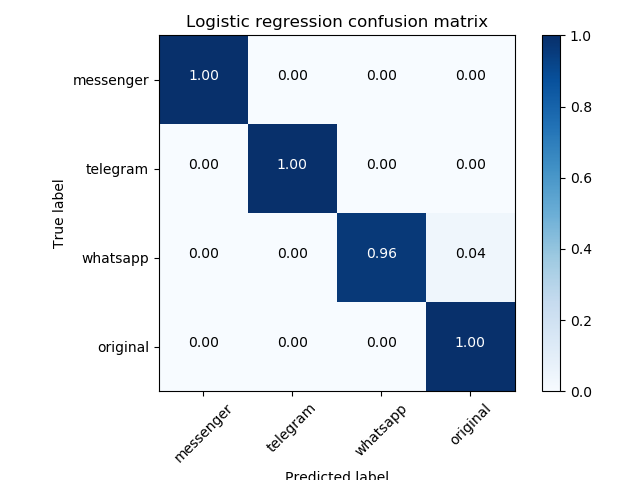
\includegraphics[scale=.6]{images/lr_initial.png} 
\caption{logistic regression} 
\end{figure} 


Result of the KFold validation with 10 bins:
 {\def\arraystretch{1.3} 
 \begin{table}[H] 
\centering 
\begin{tabular}{|l |l |l |l |l |l |l |l |l |l |}  
\hline 
1.0000&
0.9898&
0.9898&
1.0000&
1.0000&
0.9796&
0.9898&
1.0000&
0.9898&
1.0000\\ \hline  

\end{tabular} 
\end{table} }

The mean is : 0.993878\section{Linear Support Vector Machine results:}Confusion matrix with number of sample and with normalization:
 {\def\arraystretch{1.3} 
 \begin{table}[H] 
\centering 
\begin{tabular}{|l|l|l|l|l|} 
\hline 
  &messenger  &telegram  &whatsapp  &original  \\ \hline
messenger  &100  &0  &0  &0  \\ \hline
telegram  &0  &106  &0  &0  \\ \hline
whatsapp  &0  &0  &103  &4  \\ \hline
original  &0  &0  &0  &107  \\ \hline
\end{tabular} 
\end{table} }

 \begin{figure}[H] 
\centering 
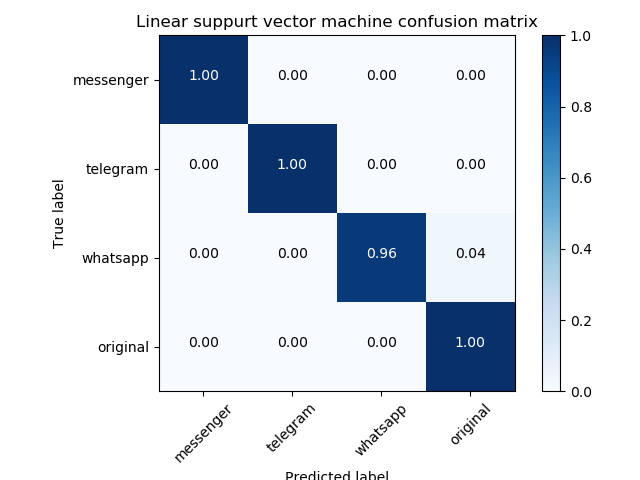
\includegraphics[scale=.6]{images/lsvm_initial.png} 
\caption{linear SVM} 
\end{figure} 


Result of the KFold validation with 10 bins:
 {\def\arraystretch{1.3} 
 \begin{table}[H] 
\centering 
\begin{tabular}{|l |l |l |l |l |l |l |l |l |l |}  
\hline 
1.0000&
0.9898&
1.0000&
1.0000&
1.0000&
0.9898&
0.9898&
1.0000&
0.9898&
1.0000\\ \hline  

\end{tabular} 
\end{table} }

The mean is : 0.995918\section{Random forest results:}Confusion matrix with number of sample and with normalization:
 {\def\arraystretch{1.3} 
 \begin{table}[H] 
\centering 
\begin{tabular}{|l|l|l|l|l|} 
\hline 
  &messenger  &telegram  &whatsapp  &original  \\ \hline
messenger  &100  &0  &0  &0  \\ \hline
telegram  &0  &106  &0  &0  \\ \hline
whatsapp  &0  &0  &103  &4  \\ \hline
original  &0  &0  &0  &107  \\ \hline
\end{tabular} 
\end{table} }

 \begin{figure}[H] 
\centering 
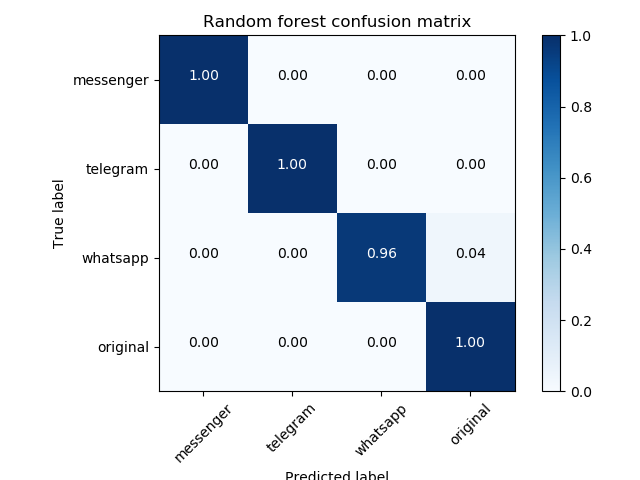
\includegraphics[scale=.6]{images/rf_initial.png} 
\caption{random forest} 
\end{figure} 


Result of the KFold validation with 10 bins:
 {\def\arraystretch{1.3} 
 \begin{table}[H] 
\centering 
\begin{tabular}{|l |l |l |l |l |l |l |l |l |l |}  
\hline 
0.9898&
0.9898&
1.0000&
1.0000&
1.0000&
0.9796&
0.9898&
1.0000&
0.9898&
1.0000\\ \hline  

\end{tabular} 
\end{table} }

The mean is : 0.993878

\chapter{Single Scenario Classification, Circularly Validation}

Here was used the same dataset as before but the training used a 0.3 of the dataset, and it is shifted circulary to cover all the dataset.Here is the table of all steps calculated \\
\begin{longtable} 
{|l |l |l |l |} 
\hline 
step  &logistic  &linear SVM  &random fo.  \\ \hline
0  &0.9831894364316239  &0.9791077839737224  &0.9870578936968979  \\ \hline
1  &0.9853026547006402  &0.9783844889010689  &0.9870578936968979  \\ \hline
2  &0.9853026547006402  &0.9775285159568015  &0.9909805452235539  \\ \hline
3  &0.9853026547006402  &0.9783844889010689  &0.9890580733784273  \\ \hline
4  &0.9871718848829855  &0.9783844889010689  &0.9890580733784273  \\ \hline
5  &0.981755684822845  &0.9908606639439437  &0.989920141798295  \\ \hline
6  &0.981755684822845  &0.9908606639439437  &0.989920141798295  \\ \hline
7  &0.981755684822845  &0.9908606639439437  &0.9888995950885928  \\ \hline
8  &0.981755684822845  &0.9908606639439437  &0.989920141798295  \\ \hline
9  &0.9797774593441748  &0.9846882267380576  &0.9836765977536278  \\ \hline
10  &0.9807773613945863  &0.9857299945019243  &0.9826969666799417  \\ \hline
11  &0.9807773613945863  &0.9846882267380576  &0.9826969666799417  \\ \hline
12  &0.9817853927299603  &0.9846882267380576  &0.9837044820834663  \\ \hline
13  &0.9817853927299603  &0.9857299945019243  &0.980725773647614  \\ \hline
14  &0.9817853927299603  &0.9857299945019243  &0.9817251354156551  \\ \hline
15  &0.9828271604938271  &0.9857299945019243  &0.9827641540487163  \\ \hline
16  &0.9828271604938271  &0.9857299945019243  &0.9827877082098887  \\ \hline
17  &0.9809303350970018  &0.9809303350970018  &0.9799310434556336  \\ \hline
18  &0.9809303350970018  &0.9809303350970018  &0.9799310434556336  \\ \hline
19  &0.9809303350970018  &0.9809303350970018  &0.9769817171132961  \\ \hline
20  &0.9809303350970018  &0.9809303350970018  &0.9799310434556336  \\ \hline
21  &0.9809303350970018  &0.9809303350970018  &0.9769817171132961  \\ \hline
22  &0.9779061415486145  &0.9799140749344002  &0.97795683313976  \\ \hline
23  &0.9779061415486145  &0.978906043599026  &0.9744170161392807  \\ \hline
24  &0.9779061415486145  &0.978906043599026  &0.9713928225908935  \\ \hline
25  &0.9779061415486145  &0.9779067519576579  &0.9769817171132961  \\ \hline
26  &0.9769068499072464  &0.9779067519576579  &0.9713928225908935  \\ \hline
27  &0.9820489340633134  &0.9849476193424314  &0.9820489340633134  \\ \hline
28  &0.9820489340633134  &0.9849476193424314  &0.9832038974293551  \\ \hline
29  &0.9820489340633134  &0.9808709993428069  &0.9801797038809681  \\ \hline
30  &0.9820489340633134  &0.9799805623885003  &0.9850731276117004  \\ \hline
31  &0.9820489340633134  &0.9799805623885003  &0.9850731276117004  \\ \hline
32  &0.9810570633546724  &0.9799144970334153  &0.9729849311036389  \\ \hline
33  &0.9627812747783722  &0.9583378598311828  &0.9542004398105941  \\ \hline
34  &0.953283825521887  &0.9489212587825018  &0.953283825521887  \\ \hline
35  &0.953283825521887  &0.9521822193250765  &0.9332107165025093  \\ \hline
36  &0.9521336702615147  &0.9510715431596557  &0.9342712270274949  \\ \hline
37  &0.9553966439474894  &0.9586655168859602  &0.941807112194959  \\ \hline
38  &0.9550624888401142  &0.9501411675781424  &0.941807112194959  \\ \hline
39  &0.9508728056918877  &0.957897835375157  &0.9435515300577979  \\ \hline
40  &0.949001628304907  &0.9569165446997437  &0.9426760297719203  \\ \hline
41  &0.949001628304907  &0.9570023590744005  &0.9426760297719203  \\ \hline
42  &0.9518168607439983  &0.9570023590744005  &0.9426760297719203  \\ \hline
43  &0.9628462719278571  &0.9690702601489536  &0.9670237271116444  \\ \hline
44  &0.9641308448001574  &0.9690415311211439  &0.9735226067675696  \\ \hline
45  &0.9611971340022054  &0.9540513512651186  &0.9735226067675696  \\ \hline
46  &0.9636358185061074  &0.9539595767948307  &0.9691897607151013  \\ \hline
47  &0.9634237045681469  &0.9549009600982763  &0.9713033424446343  \\ \hline
48  &0.9630416021422119  &0.9457796737082027  &0.9724089271961905  \\ \hline
49  &0.9590950950950952  &0.9645468263150108  &0.9631028529724224  \\ \hline
50  &0.9590950950950952  &0.9645468263150108  &0.9651904231493449  \\ \hline
51  &0.9590950950950952  &0.9645468263150108  &0.9651904231493449  \\ \hline
52  &0.9590950950950952  &0.9645468263150108  &0.9651904231493449  \\ \hline
53  &0.9704082737708469  &0.9750147841513898  &0.9745533102297715  \\ \hline
54  &0.9749984999849999  &0.9794007490636705  &0.9800443458980044  \\ \hline
55  &0.9749984999849999  &0.9794007490636705  &0.9778754788737738  \\ \hline
56  &0.9749984999849999  &0.9794007490636705  &0.9789560728306903  \\ \hline
57  &0.9765285344002652  &0.9802631578947368  &0.9790280857354028  \\ \hline
58  &0.9775769230769231  &0.9802631578947368  &0.9779480414953162  \\ \hline
59  &0.9775769230769231  &0.9802631578947368  &0.9791724190826814  \\ \hline
60  &0.9756841360427018  &0.978544776119403  &0.9780137313157126  \\ \hline
61  &0.9757692307692307  &0.978544776119403  &0.9780893448656607  \\ \hline
62  &0.9746787205323791  &0.9794007490636705  &0.980188679245283  \\ \hline
63  &0.9959839357429718  &0.9989837398373984  &0.9989837398373984  \\ \hline
64  &0.9899551291586098  &0.9949676755803702  &0.9898723422423363  \\ \hline
65  &0.9814065924422243  &0.989179818268771  &0.9850946868966615  \\ \hline
66  &0.9851206921404461  &0.989179818268771  &0.9881081682594579  \\ \hline
67  &0.983242407923623  &0.9801158153090965  &0.9831320060410063  \\ \hline
68  &0.9841779184557378  &0.9791077839737224  &0.9900154191754695  \\ \hline
69  &0.9841779184557378  &0.9791077839737224  &0.987165432614862  \\ \hline
\end{longtable} 
Average of all steps: 

 {\def\arraystretch{1.3} 
 \begin{table}[H] 
\centering 
\begin{tabular}{|l|l|l|} 
\hline 
logistic r.  &linear SVM  &random f.  \\ \hline
0.9742098967923488  &0.9754435548603985  &0.9748451176133341  \\ \hline
\end{tabular} 
\end{table} }
Confusion matrix estimated on overall tests: 

 \begin{figure}[H] 
\centering 
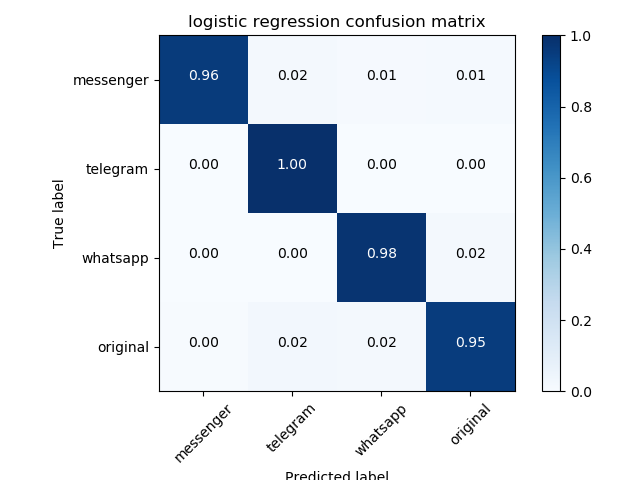
\includegraphics[scale=.6]{images/logistic_total.png} 
\caption{logistic regression} 
\end{figure} 

 \begin{figure}[H] 
\centering 
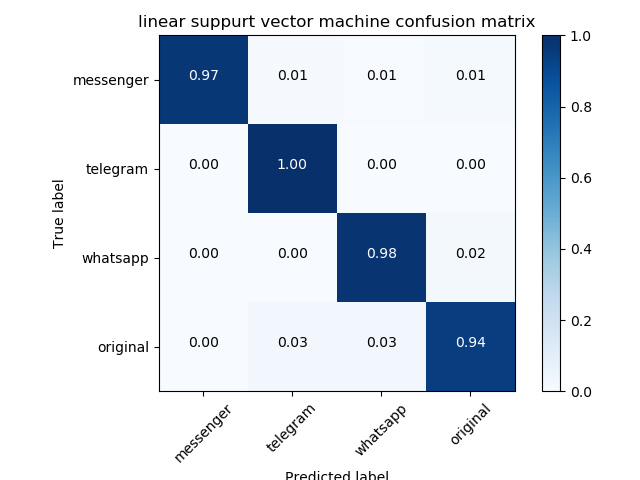
\includegraphics[scale=.6]{images/lsvm_total.png} 
\caption{linear SVM} 
\end{figure} 

 \begin{figure}[H] 
\centering 
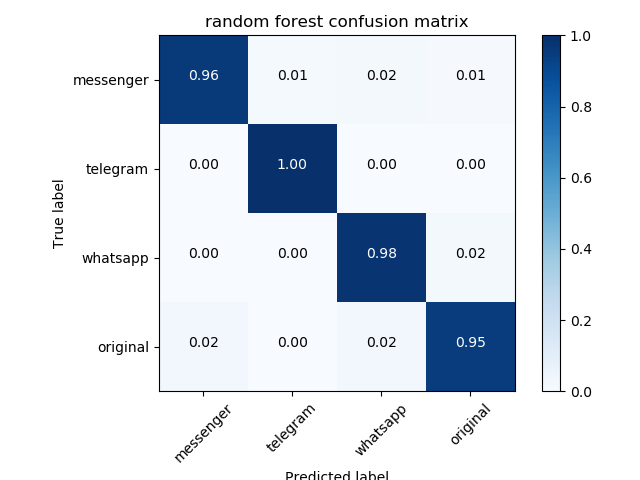
\includegraphics[scale=.6]{images/random_total.png} 
\caption{random forest} 
\end{figure} 

	\chapter{Single Scenario Classification, KFold Validation}

Starting with fitting randomly the classifiers, there are some statistics of the data used for the first test: \\
 {\def\arraystretch{1.3} 
 \begin{table}[H] 
\centering 
\begin{tabular}{|l|l|l|} 
\hline 
  &count train  &count test  \\ \hline
messenger  &249  &100  \\ \hline
telegram  &244  &106  \\ \hline
whatsapp  &243  &107  \\ \hline
original  &243  &107  \\ \hline
\end{tabular} 
\end{table} }
\section{Logistic regression results:} 
Confusion matrix with number of sample and with normalization:
 {\def\arraystretch{1.3} 
 \begin{table}[H] 
\centering 
\begin{tabular}{|l|l|l|l|l|} 
\hline 
  &messenger  &telegram  &whatsapp  &original  \\ \hline
messenger  &100  &0  &0  &0  \\ \hline
telegram  &0  &106  &0  &0  \\ \hline
whatsapp  &0  &0  &103  &4  \\ \hline
original  &0  &0  &0  &107  \\ \hline
\end{tabular} 
\end{table} }

 \begin{figure}[H] 
\centering 
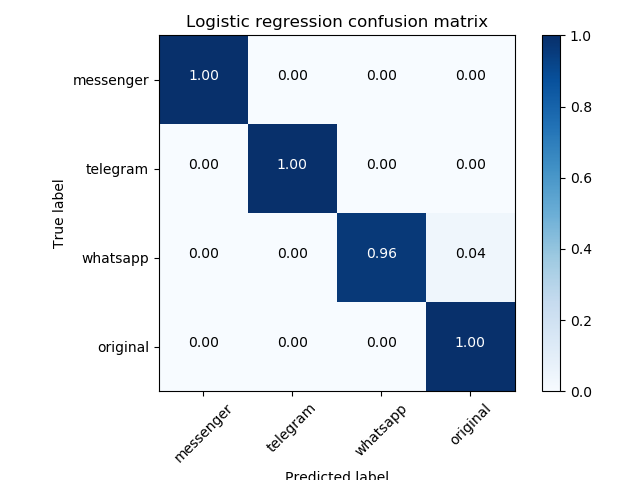
\includegraphics[scale=.6]{images/lr_initial.png} 
\caption{logistic regression} 
\end{figure} 


Result of the KFold validation with 10 bins:
 {\def\arraystretch{1.3} 
 \begin{table}[H] 
\centering 
\begin{tabular}{|l |l |l |l |l |l |l |l |l |l |}  
\hline 
0.9796&
0.9898&
1.0000&
1.0000&
1.0000&
0.9898&
0.9898&
1.0000&
0.9898&
1.0000\\ \hline  

\end{tabular} 
\end{table} }

The mean is : 0.993878\section{Linear Support Vector Machine results:}Confusion matrix with number of sample and with normalization:
 {\def\arraystretch{1.3} 
 \begin{table}[H] 
\centering 
\begin{tabular}{|l|l|l|l|l|} 
\hline 
  &messenger  &telegram  &whatsapp  &original  \\ \hline
messenger  &100  &0  &0  &0  \\ \hline
telegram  &0  &106  &0  &0  \\ \hline
whatsapp  &0  &0  &103  &4  \\ \hline
original  &0  &0  &0  &107  \\ \hline
\end{tabular} 
\end{table} }

 \begin{figure}[H] 
\centering 
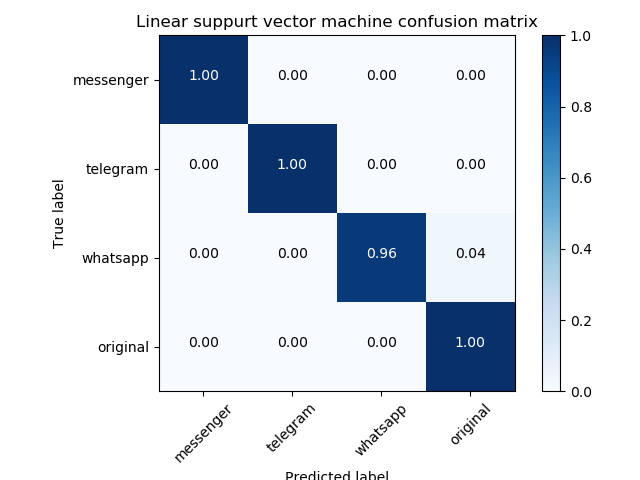
\includegraphics[scale=.6]{images/lsvm_initial.png} 
\caption{linear SVM} 
\end{figure} 


Result of the KFold validation with 10 bins:
 {\def\arraystretch{1.3} 
 \begin{table}[H] 
\centering 
\begin{tabular}{|l |l |l |l |l |l |l |l |l |l |}  
\hline 
0.9898&
0.9898&
1.0000&
1.0000&
1.0000&
0.9796&
0.9898&
1.0000&
0.9898&
1.0000\\ \hline  

\end{tabular} 
\end{table} }

The mean is : 0.993878\section{Random forest results:}Confusion matrix with number of sample and with normalization:
 {\def\arraystretch{1.3} 
 \begin{table}[H] 
\centering 
\begin{tabular}{|l|l|l|l|l|} 
\hline 
  &messenger  &telegram  &whatsapp  &original  \\ \hline
messenger  &100  &0  &0  &0  \\ \hline
telegram  &0  &106  &0  &0  \\ \hline
whatsapp  &0  &0  &103  &4  \\ \hline
original  &0  &0  &0  &107  \\ \hline
\end{tabular} 
\end{table} }

 \begin{figure}[H] 
\centering 
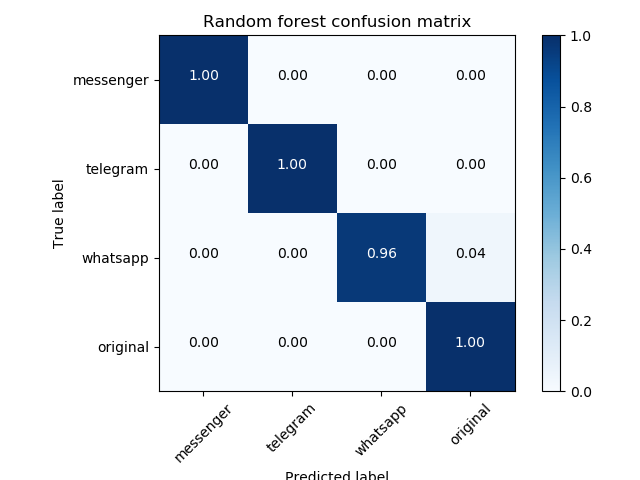
\includegraphics[scale=.6]{images/rf_initial.png} 
\caption{random forest} 
\end{figure} 


Result of the KFold validation with 10 bins:
 {\def\arraystretch{1.3} 
 \begin{table}[H] 
\centering 
\begin{tabular}{|l |l |l |l |l |l |l |l |l |l |}  
\hline 
1.0000&
0.9898&
1.0000&
1.0000&
1.0000&
0.9796&
0.9898&
1.0000&
0.9898&
0.9897\\ \hline  

\end{tabular} 
\end{table} }

The mean is : 0.993867

\chapter{Single Scenario Classification, Circularly Validation}

Here was used the same dataset as before but the training used a 0.3 of the dataset, and it is shifted circulary to cover all the dataset.Here is the table of all steps calculated \\
\begin{longtable} 
{|l |l |l |l |} 
\hline 
step  &logistic  &linear SVM  &random fo.  \\ \hline
0  &0.989179818268771  &0.9861800141743444  &0.9901213241201993  \\ \hline
1  &0.9848642886352729  &0.989179818268771  &0.9901086744322249  \\ \hline
2  &0.9859958494970797  &0.989179818268771  &0.992039295392954  \\ \hline
3  &0.9840239043824701  &0.989179818268771  &0.9879411617983916  \\ \hline
4  &0.9838346881813623  &0.989179818268771  &0.9878321961314647  \\ \hline
5  &0.9850775862706985  &0.9888435941925785  &0.9929795918367347  \\ \hline
6  &0.9849757394589151  &0.9899004065040651  &0.989900983984118  \\ \hline
7  &0.9869068386254386  &0.9899004065040651  &0.99103468547913  \\ \hline
8  &0.9859149679167976  &0.9899004065040651  &0.990969961616947  \\ \hline
9  &0.9826572092251535  &0.9861966137690223  &0.9817251354156551  \\ \hline
10  &0.9847290722474007  &0.9870545842786601  &0.9827326856656295  \\ \hline
11  &0.9837185571115683  &0.9857771334299855  &0.9846840787373938  \\ \hline
12  &0.9838354913678619  &0.9859658778205833  &0.9846840787373938  \\ \hline
13  &0.9813181579293129  &0.9861166500498505  &0.9807610095111248  \\ \hline
14  &0.9813181579293129  &0.9853611471537412  &0.9787703014260097  \\ \hline
15  &0.9831900496861925  &0.9862857095347368  &0.980725773647614  \\ \hline
16  &0.9841168266469769  &0.9862857095347368  &0.9808059618649602  \\ \hline
17  &0.9822572998070824  &0.9822572998070824  &0.9760144649257553  \\ \hline
18  &0.9821251322105606  &0.9822572998070824  &0.97795683313976  \\ \hline
19  &0.9820101172758178  &0.982107843137255  &0.9750549818320903  \\ \hline
20  &0.9820101172758178  &0.9826435137223949  &0.9769817171132961  \\ \hline
21  &0.9820101172758178  &0.9822440033492588  &0.9769817171132961  \\ \hline
22  &0.9820101172758178  &0.9819674282059272  &0.9769817171132961  \\ \hline
23  &0.9789859263543474  &0.9826435137223949  &0.9734258819806992  \\ \hline
24  &0.9789859263543474  &0.9844528594528594  &0.9734258819806992  \\ \hline
25  &0.9790240688968155  &0.9835470085470086  &0.9734258819806992  \\ \hline
26  &0.978963179539905  &0.9808615772912023  &0.9734258819806992  \\ \hline
27  &0.981011696187139  &0.9881608339538348  &0.981094861660079  \\ \hline
28  &0.9809466587092924  &0.9880438882784184  &0.981094861660079  \\ \hline
29  &0.978957428886153  &0.9869016393442622  &0.981094861660079  \\ \hline
30  &0.9771308523409363  &0.9880438882784184  &0.981094861660079  \\ \hline
31  &0.9839638554216867  &0.9889326989562411  &0.981094861660079  \\ \hline
32  &0.9821736011477762  &0.9839576074332173  &0.974576923076923  \\ \hline
33  &0.9632234670976825  &0.963381121890158  &0.9618357875948238  \\ \hline
34  &0.955915762290795  &0.9604524917457968  &0.9523383383383384  \\ \hline
35  &0.9558080031175651  &0.9615025224051383  &0.9332107165025093  \\ \hline
36  &0.9537713472485769  &0.9616828738173668  &0.9342712270274949  \\ \hline
37  &0.9567246849068246  &0.9705229237156167  &0.941807112194959  \\ \hline
38  &0.9624805441127516  &0.9689582071471836  &0.941807112194959  \\ \hline
39  &0.9656916766799837  &0.9754108565737052  &0.9426760297719203  \\ \hline
40  &0.9645393196105017  &0.9744245524296675  &0.9426760297719203  \\ \hline
41  &0.9674626293689195  &0.9725627105089125  &0.9426760297719203  \\ \hline
42  &0.9654192933722927  &0.970744883788362  &0.9435515300577979  \\ \hline
43  &0.9695591349062311  &0.9723367392625123  &0.9638905905957089  \\ \hline
44  &0.9684887580521552  &0.9724221573471613  &0.9735226067675696  \\ \hline
45  &0.968972132612202  &0.9742295202245372  &0.9713033424446343  \\ \hline
46  &0.9682197824252712  &0.9742295202245372  &0.9735226067675696  \\ \hline
47  &0.9693788613812181  &0.9731363489522036  &0.9724089271961905  \\ \hline
48  &0.9668187320808225  &0.9683336860555347  &0.9713033424446343  \\ \hline
49  &0.9642240738507779  &0.9642997792344016  &0.9631028529724224  \\ \hline
50  &0.9629520363275152  &0.9642997792344016  &0.9641429955913738  \\ \hline
51  &0.9631771897864273  &0.9642997792344016  &0.9609153080205712  \\ \hline
52  &0.9643385011275081  &0.9642997792344016  &0.9651904231493449  \\ \hline
53  &0.9738195798137318  &0.9726644779063561  &0.9702353383569476  \\ \hline
54  &0.9782388663967612  &0.9752631578947368  &0.9778754788737738  \\ \hline
55  &0.9782388663967612  &0.9695209703947368  &0.9778754788737738  \\ \hline
56  &0.9782388663967612  &0.9713281539030707  &0.9800443458980044  \\ \hline
57  &0.9789586940956656  &0.9714048901782014  &0.9789560728306903  \\ \hline
58  &0.9808488835137682  &0.9750631313131313  &0.980188679245283  \\ \hline
59  &0.9809913155949741  &0.9854702263238849  &0.9790973762010348  \\ \hline
60  &0.9820075757575757  &0.9808654423423285  &0.9800443458980044  \\ \hline
61  &0.9820075757575757  &0.9820075757575757  &0.9800443458980044  \\ \hline
62  &0.9820075757575757  &0.9820075757575757  &0.9780137313157126  \\ \hline
63  &1.0  &1.0  &0.9989837398373984  \\ \hline
64  &0.9949551291586097  &0.9939669421487604  &0.9858662941153005  \\ \hline
65  &0.9901960784313726  &0.9892578125  &0.9831053292616855  \\ \hline
66  &0.9901960784313726  &0.9892578125  &0.9898912530352956  \\ \hline
67  &0.9901960784313726  &0.9892578125  &0.9920351473922903  \\ \hline
68  &0.9881717869333969  &0.9852417482429718  &0.986020872302839  \\ \hline
69  &0.9881717869333969  &0.9861800141743444  &0.9910744534968137  \\ \hline
\end{longtable} 
Average of all steps: 

 {\def\arraystretch{1.3} 
 \begin{table}[H] 
\centering 
\begin{tabular}{|l|l|l|} 
\hline 
logistic r.  &linear SVM  &random f.  \\ \hline
0.9777519138070937  &0.9801399772382293  &0.9746721183192149  \\ \hline
\end{tabular} 
\end{table} }
Confusion matrix estimated on overall tests: 

 \begin{figure}[H] 
\centering 
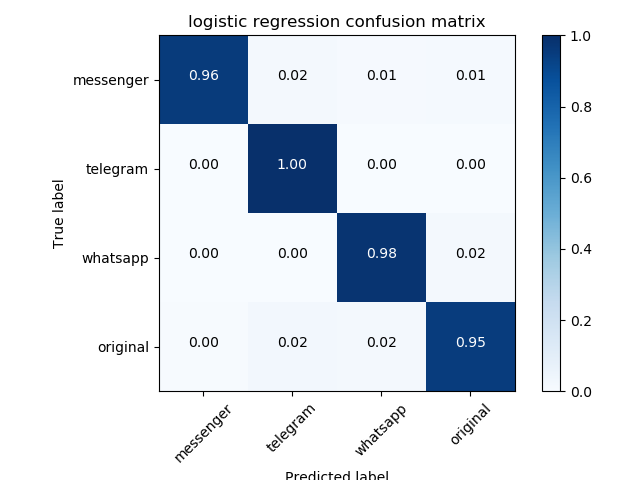
\includegraphics[scale=.6]{images/logistic_total.png} 
\caption{logistic regression} 
\end{figure} 

 \begin{figure}[H] 
\centering 
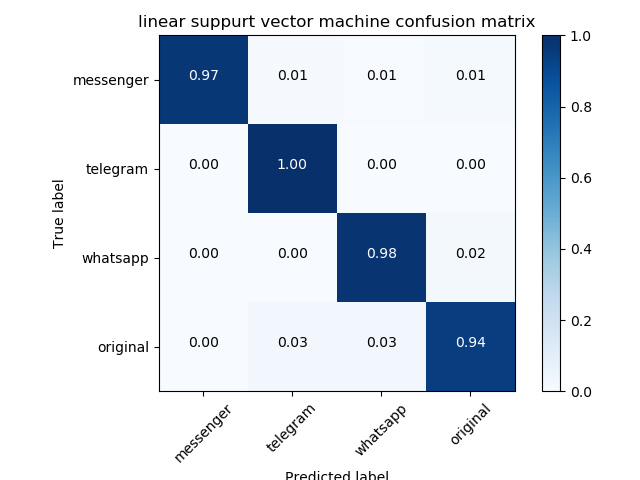
\includegraphics[scale=.6]{images/lsvm_total.png} 
\caption{linear SVM} 
\end{figure} 

 \begin{figure}[H] 
\centering 
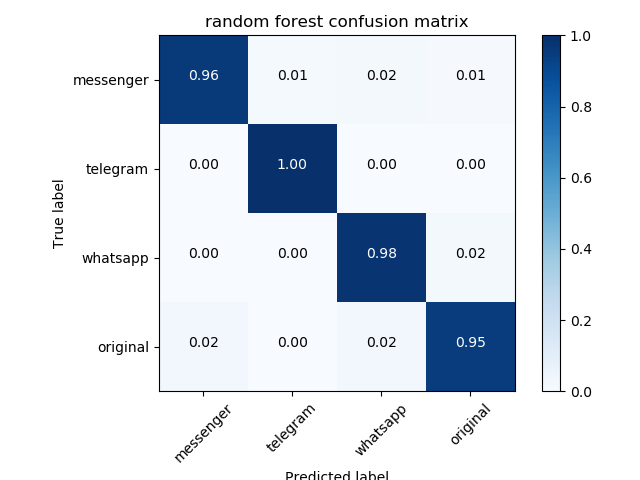
\includegraphics[scale=.6]{images/random_total.png} 
\caption{random forest} 
\end{figure} 

	%\input{report_double}
	%\input{flow}
	\chapter{Double Scenario Classification of the last shared app, KFold Validation}Starting with fitting randomly the classifiers, there are some statistics of the data used for the first test: \\
 {\def\arraystretch{1.3} 
 \begin{table}[H] 
\centering 
\begin{tabular}{|l|l|l|} 
\hline 
  &count train  &count test  \\ \hline
messenger  &302  &748  \\ \hline
telegram  &314  &736  \\ \hline
whatsapp  &340  &710  \\ \hline
original  &94  &256  \\ \hline
\end{tabular} 
\end{table} }
\section{Logistic regression results:} 
Confusion matrix with number of sample and with normalization:
 {\def\arraystretch{1.3} 
 \begin{table}[H] 
\centering 
\begin{tabular}{|l|l|l|l|l|} 
\hline 
  &messenger  &telegram  &whatsapp  &original  \\ \hline
messenger  &741  &0  &7  &0  \\ \hline
telegram  &0  &676  &60  &0  \\ \hline
whatsapp  &1  &226  &480  &3  \\ \hline
original  &0  &0  &8  &248  \\ \hline
\end{tabular} 
\end{table} }

 \begin{figure}[H] 
\centering 
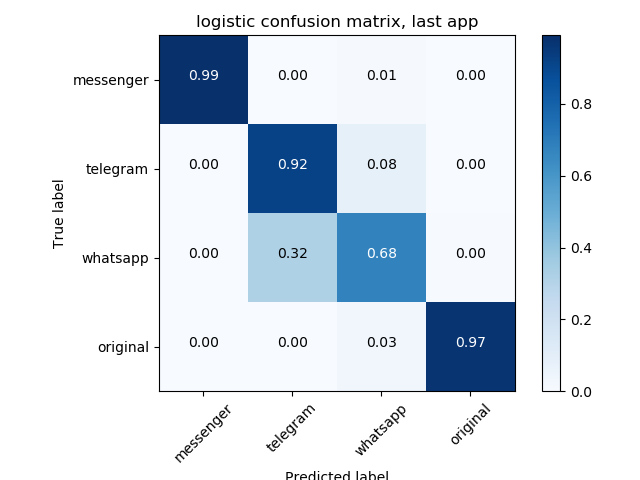
\includegraphics[scale=.6]{images/lr_initial_double_simple.png} 
\caption{logistic regression, last app classified} 
\end{figure} 


Result of the KFold validation with 10 bins:
 {\def\arraystretch{1.3} 
 \begin{table}[H] 
\centering 
\begin{tabular}{|l |l |l |l |l |l |l |l |l |l |}  
\hline 
0.9048&
0.8190&
0.9143&
0.8571&
0.8476&
0.9429&
0.8857&
0.9048&
0.8381&
0.8762\\ \hline  

\end{tabular} 
\end{table} }

The mean is : 0.879048\section{Linear Support Vector Machine results:} 
Confusion matrix with number of sample and with normalization:
 {\def\arraystretch{1.3} 
 \begin{table}[H] 
\centering 
\begin{tabular}{|l|l|l|l|l|} 
\hline 
  &messenger  &telegram  &whatsapp  &original  \\ \hline
messenger  &740  &1  &7  &0  \\ \hline
telegram  &0  &601  &135  &0  \\ \hline
whatsapp  &1  &202  &504  &3  \\ \hline
original  &0  &0  &8  &248  \\ \hline
\end{tabular} 
\end{table} }

 \begin{figure}[H] 
\centering 
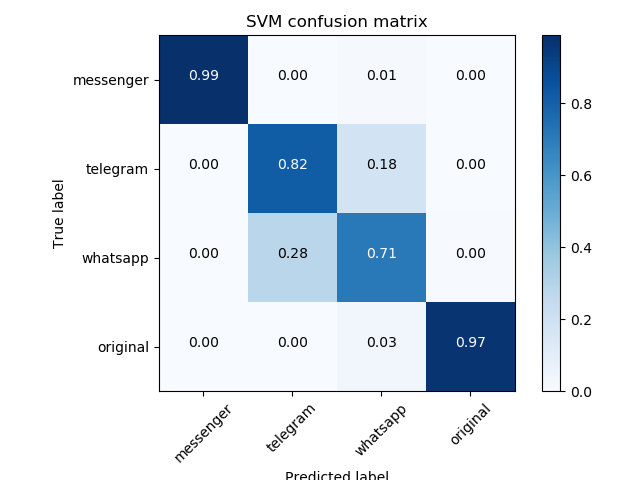
\includegraphics[scale=.6]{images/lsvm_initial_double_simple.png} 
\caption{linear SVM, last app classified} 
\end{figure} 


Result of the KFold validation with 10 bins:
 {\def\arraystretch{1.3} 
 \begin{table}[H] 
\centering 
\begin{tabular}{|l |l |l |l |l |l |l |l |l |l |}  
\hline 
0.8381&
0.7905&
0.8762&
0.8667&
0.8190&
0.8857&
0.8381&
0.8762&
0.8000&
0.8571\\ \hline  

\end{tabular} 
\end{table} }

The mean is : 0.844762\section{Random forest results:} 
Confusion matrix with number of sample and with normalization:
 {\def\arraystretch{1.3} 
 \begin{table}[H] 
\centering 
\begin{tabular}{|l|l|l|l|l|} 
\hline 
  &messenger  &telegram  &whatsapp  &original  \\ \hline
messenger  &743  &0  &5  &0  \\ \hline
telegram  &0  &589  &147  &0  \\ \hline
whatsapp  &1  &233  &473  &3  \\ \hline
original  &1  &0  &2  &253  \\ \hline
\end{tabular} 
\end{table} }

 \begin{figure}[H] 
\centering 
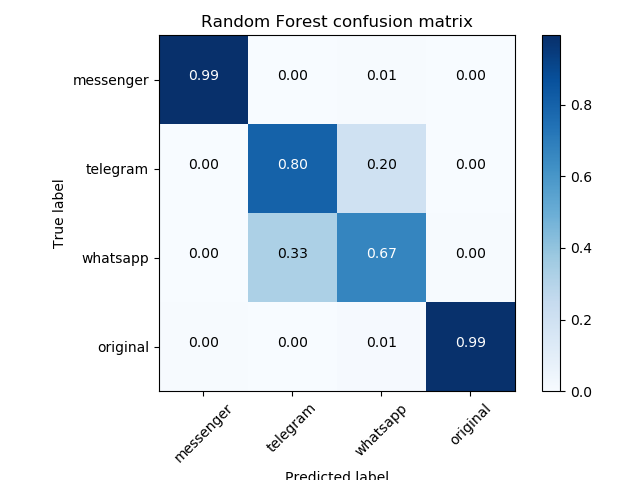
\includegraphics[scale=.6]{images/rf_initial_double_simple.png} 
\caption{random forest, last app classified} 
\end{figure} 


Result of the KFold validation with 10 bins:
 {\def\arraystretch{1.3} 
 \begin{table}[H] 
\centering 
\begin{tabular}{|l |l |l |l |l |l |l |l |l |l |}  
\hline 
0.8286&
0.8190&
0.8762&
0.8952&
0.8381&
0.8762&
0.8286&
0.8476&
0.8571&
0.8381\\ \hline  

\end{tabular} 
\end{table} }

The mean is : 0.850476
	

\chapter{Double Scenario Classification of the first and last shared app, KFold Validation}

Starting with fitting randomly the classifiers, there are some statistics of the data used for the first test: \\
 {\def\arraystretch{1.3} 
 \begin{table}[H] 
\centering 
\begin{tabular}{|l|l|l|} 
\hline 
  &count train  &count test  \\ \hline
mess\_mess  &96  &254  \\ \hline
tele\_mess  &99  &251  \\ \hline
what\_mess  &107  &243  \\ \hline
mess\_tele  &98  &252  \\ \hline
tele\_tele  &111  &239  \\ \hline
what\_tele  &105  &245  \\ \hline
mess\_what  &116  &234  \\ \hline
tele\_what  &103  &247  \\ \hline
what\_what  &121  &229  \\ \hline
original  &94  &256  \\ \hline
\end{tabular} 
\end{table} }
\section{Logistic regression results:} 
Confusion matrix with number of sample and with normalization:
 {\def\arraystretch{1.3} 
 \begin{table}[H] 
\centering 
\begin{tabular}{|l|l|l|l|l|l|l|l|l|l|l|} 
\hline 
  &m\_m  &m\_t  &m\_w  &t\_m  &t\_t  &t\_w  &w\_m  &w\_t  &w\_w  &original  \\ \hline
mess\_mess  &249  &4  &1  &0  &0  &0  &0  &0  &0  &0  \\ \hline
tele\_mess  &0  &241  &9  &0  &1  &0  &0  &0  &0  &0  \\ \hline
what\_mess  &21  &9  &213  &0  &0  &0  &0  &0  &0  &0  \\ \hline
mess\_tele  &0  &0  &1  &43  &107  &2  &0  &99  &0  &0  \\ \hline
tele\_tele  &0  &0  &0  &52  &79  &0  &0  &108  &0  &0  \\ \hline
what\_tele  &0  &0  &0  &0  &1  &243  &0  &1  &0  &0  \\ \hline
mess\_what  &0  &2  &0  &0  &0  &0  &84  &2  &146  &0  \\ \hline
tele\_what  &0  &0  &0  &57  &112  &0  &0  &78  &0  &0  \\ \hline
what\_what  &0  &0  &0  &0  &0  &0  &102  &0  &124  &3  \\ \hline
original  &1  &0  &0  &0  &0  &0  &0  &0  &4  &251  \\ \hline
\end{tabular} 
\end{table} }

 \begin{figure}[H] 
\centering 
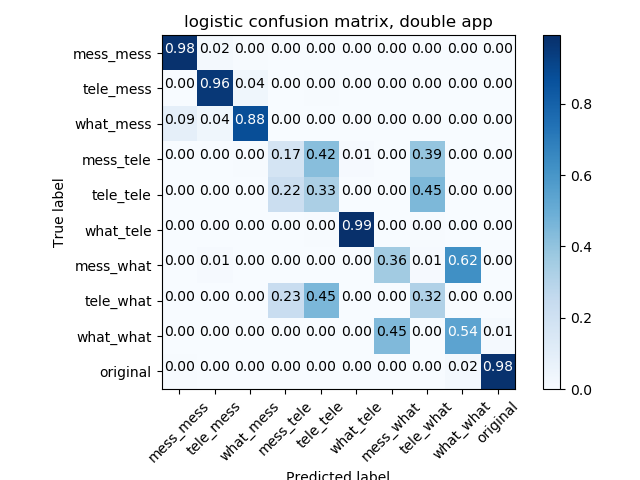
\includegraphics[scale=.6]{images/lr_initial_double_complete.png} 
\caption{logistic regression, last app classified} 
\end{figure} 


Result of the KFold validation with 10 bins:
 {\def\arraystretch{1.3} 
 \begin{table}[H] 
\centering 
\begin{tabular}{|l |l |l |l |l |l |l |l |l |l |}  
\hline 
0.5905&
0.5905&
0.6571&
0.6190&
0.5810&
0.6476&
0.7048&
0.6762&
0.6190&
0.6762\\ \hline  

\end{tabular} 
\end{table} }

The mean is : 0.636190\section{Linear Support Vector Machine results:} 
Confusion matrix with number of sample and with normalization:
 {\def\arraystretch{1.3} 
 \begin{table}[H] 
\centering 
\begin{tabular}{|l|l|l|l|l|l|l|l|l|l|l|} 
\hline 
  &m\_m  &m\_t  &m\_w  &t\_m  &t\_t  &t\_w  &w\_m  &w\_t  &w\_w  &original  \\ \hline
mess\_mess  &246  &3  &2  &0  &0  &0  &2  &0  &0  &1  \\ \hline
tele\_mess  &0  &233  &9  &0  &4  &0  &2  &0  &3  &0  \\ \hline
what\_mess  &22  &5  &209  &3  &0  &4  &0  &0  &0  &0  \\ \hline
mess\_tele  &0  &0  &0  &47  &102  &1  &0  &101  &1  &0  \\ \hline
tele\_tele  &0  &0  &0  &55  &58  &4  &0  &122  &0  &0  \\ \hline
what\_tele  &0  &0  &0  &1  &0  &244  &0  &0  &0  &0  \\ \hline
mess\_what  &0  &1  &0  &0  &0  &0  &90  &2  &141  &0  \\ \hline
tele\_what  &0  &0  &0  &58  &108  &3  &0  &78  &0  &0  \\ \hline
what\_what  &0  &0  &0  &0  &0  &0  &114  &0  &112  &3  \\ \hline
original  &0  &0  &0  &0  &1  &0  &1  &0  &8  &246  \\ \hline
\end{tabular} 
\end{table} }

 \begin{figure}[H] 
\centering 
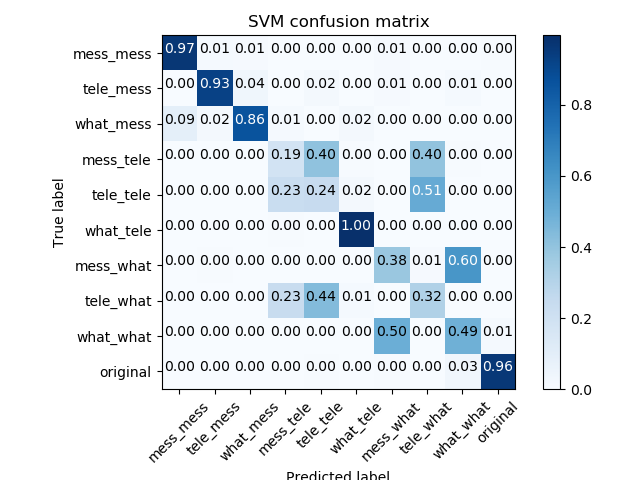
\includegraphics[scale=.6]{images/lsvm_initial_double_complete.png} 
\caption{linear SVM, last app classified} 
\end{figure} 


Result of the KFold validation with 10 bins:
 {\def\arraystretch{1.3} 
 \begin{table}[H] 
\centering 
\begin{tabular}{|l |l |l |l |l |l |l |l |l |l |}  
\hline 
0.5905&
0.5619&
0.6857&
0.6000&
0.5429&
0.6286&
0.6762&
0.6667&
0.5810&
0.6571\\ \hline  

\end{tabular} 
\end{table} }

The mean is : 0.619048\section{Random forest results:} 
Confusion matrix with number of sample and with normalization:
 {\def\arraystretch{1.3} 
 \begin{table}[H] 
\centering 
\begin{tabular}{|l|l|l|l|l|l|l|l|l|l|l|} 
\hline 
  &m\_m  &m\_t  &m\_w  &t\_m  &t\_t  &t\_w  &w\_m  &w\_t  &w\_w  &original  \\ \hline
mess\_mess  &244  &6  &3  &0  &0  &0  &1  &0  &0  &0  \\ \hline
tele\_mess  &1  &243  &7  &0  &0  &0  &0  &0  &0  &0  \\ \hline
what\_mess  &24  &18  &193  &0  &0  &0  &2  &0  &5  &1  \\ \hline
mess\_tele  &0  &0  &0  &35  &109  &3  &0  &105  &0  &0  \\ \hline
tele\_tele  &0  &0  &0  &81  &39  &4  &0  &115  &0  &0  \\ \hline
what\_tele  &0  &0  &0  &1  &0  &243  &0  &1  &0  &0  \\ \hline
mess\_what  &0  &1  &0  &0  &0  &0  &62  &0  &171  &0  \\ \hline
tele\_what  &0  &0  &0  &80  &121  &5  &0  &41  &0  &0  \\ \hline
what\_what  &0  &0  &0  &0  &0  &0  &123  &0  &103  &3  \\ \hline
original  &0  &0  &1  &0  &0  &0  &0  &0  &2  &253  \\ \hline
\end{tabular} 
\end{table} }

 \begin{figure}[H] 
\centering 
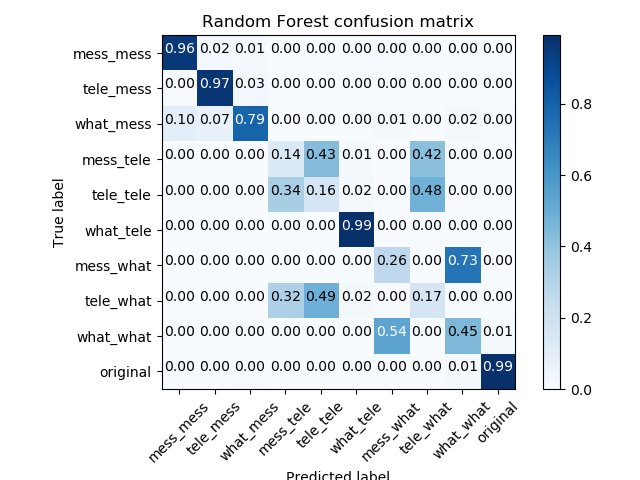
\includegraphics[scale=.6]{images/rf_initial_double_complete.png} 
\caption{random forest, last app classified} 
\end{figure} 


Result of the KFold validation with 10 bins:
 {\def\arraystretch{1.3} 
 \begin{table}[H] 
\centering 
\begin{tabular}{|l |l |l |l |l |l |l |l |l |l |}  
\hline 
0.5905&
0.5048&
0.6095&
0.6000&
0.5524&
0.6286&
0.6095&
0.6286&
0.5238&
0.6000\\ \hline  

\end{tabular} 
\end{table} }

The mean is : 0.58476229
	

\chapter{Single and double scenario, KFold Validation}

Starting with fitting randomly the classifiers, there are some statistics of the data used for the first test: \\
 {\def\arraystretch{1.3} 
 \begin{table}[H] 
\centering 
\begin{tabular}{|l|l|l|} 
\hline 
  &count train  &count test  \\ \hline
mess  &97  &253  \\ \hline
tele  &335  &715  \\ \hline
what  &219  &481  \\ \hline
mess\_mess  &99  &251  \\ \hline
tele\_mess  &113  &237  \\ \hline
what\_mess  &93  &257  \\ \hline
mess\_tele  &89  &261  \\ \hline
what\_tele  &103  &247  \\ \hline
mess\_what  &106  &244  \\ \hline
original  &111  &239  \\ \hline
\end{tabular} 
\end{table} }
\section{Logistic regression results:} 
Confusion matrix with number of sample and with normalization:
 {\def\arraystretch{1.3} 
 \begin{table}[H] 
\centering 
\begin{tabular}{|l|l|l|l|l|l|l|l|l|l|l|} 
\hline 
  &m  &t  &w  &m\_m  &m\_t  &m\_w  &t\_m  &t\_w  &w\_m  &original  \\ \hline
mess  &181  &0  &0  &45  &4  &23  &0  &0  &0  &0  \\ \hline
tele  &0  &700  &0  &0  &0  &0  &9  &6  &0  &0  \\ \hline
what  &0  &0  &414  &0  &0  &0  &0  &0  &63  &4  \\ \hline
mess\_mess  &22  &0  &0  &217  &6  &6  &0  &0  &0  &0  \\ \hline
tele\_mess  &0  &0  &0  &0  &225  &12  &0  &0  &0  &0  \\ \hline
what\_mess  &0  &0  &0  &0  &77  &180  &0  &0  &0  &0  \\ \hline
mess\_tele  &0  &248  &0  &0  &0  &0  &6  &7  &0  &0  \\ \hline
what\_tele  &0  &7  &0  &0  &0  &0  &0  &240  &0  &0  \\ \hline
mess\_what  &0  &1  &180  &0  &0  &0  &0  &0  &63  &0  \\ \hline
original  &0  &0  &0  &0  &0  &0  &0  &0  &0  &239  \\ \hline
\end{tabular} 
\end{table} }

 \begin{figure}[H] 
\centering 
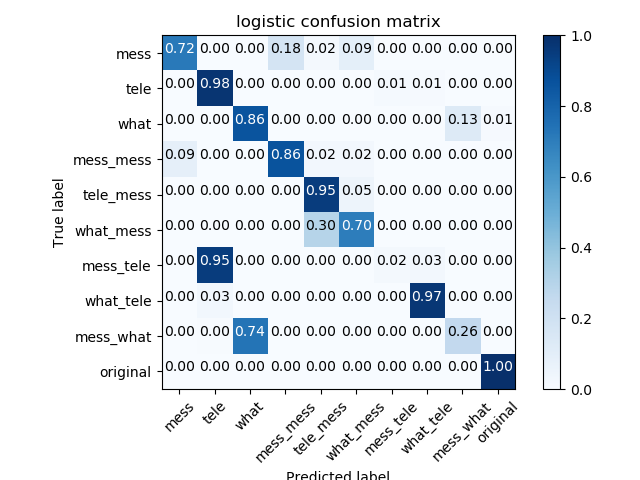
\includegraphics[scale=.6]{images/lr_initial_single_double_complete.png} 
\caption{logistic regression, last app classified} 
\end{figure} 


Result of the KFold validation with 10 bins:
 {\def\arraystretch{1.3} 
 \begin{table}[H] 
\centering 
\begin{tabular}{|l |l |l |l |l |l |l |l |l |l |}  
\hline 
0.8248&
0.8029&
0.7737&
0.8029&
0.7299&
0.8162&
0.7426&
0.8088&
0.7868&
0.8015\\ \hline  

\end{tabular} 
\end{table} }

The mean is : 0.789019\section{Linear Support Vector Machine results:} 
Confusion matrix with number of sample and with normalization:
 {\def\arraystretch{1.3} 
 \begin{table}[H] 
\centering 
\begin{tabular}{|l|l|l|l|l|l|l|l|l|l|l|} 
\hline 
  &m  &t  &w  &m\_m  &m\_t  &m\_w  &t\_m  &t\_w  &w\_m  &original  \\ \hline
mess  &195  &0  &0  &37  &4  &17  &0  &0  &0  &0  \\ \hline
tele  &0  &681  &0  &0  &0  &0  &34  &0  &0  &0  \\ \hline
what  &0  &0  &386  &0  &0  &0  &0  &0  &91  &4  \\ \hline
mess\_mess  &26  &0  &0  &217  &5  &3  &0  &0  &0  &0  \\ \hline
tele\_mess  &0  &0  &0  &0  &217  &20  &0  &0  &0  &0  \\ \hline
what\_mess  &0  &0  &1  &1  &44  &211  &0  &0  &0  &0  \\ \hline
mess\_tele  &0  &232  &0  &0  &0  &0  &29  &0  &0  &0  \\ \hline
what\_tele  &0  &5  &0  &0  &0  &0  &0  &242  &0  &0  \\ \hline
mess\_what  &0  &0  &145  &0  &1  &0  &0  &0  &98  &0  \\ \hline
original  &0  &0  &0  &0  &0  &0  &0  &0  &0  &239  \\ \hline
\end{tabular} 
\end{table} }

 \begin{figure}[H] 
\centering 
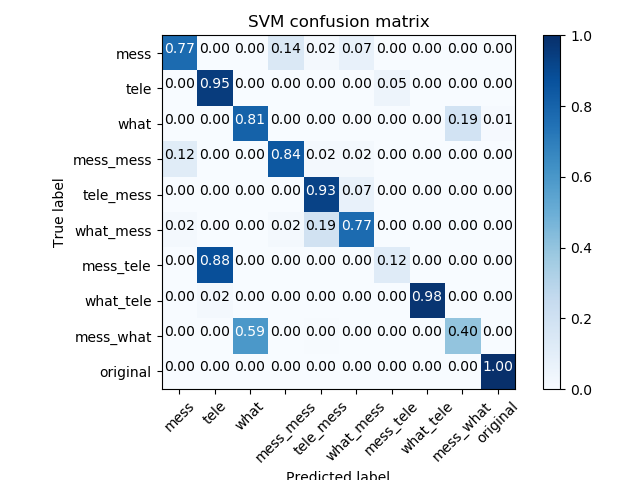
\includegraphics[scale=.6]{images/lsvm_initial_single_double_complete.png} 
\caption{linear SVM, last app classified} 
\end{figure} 


Result of the KFold validation with 10 bins:
 {\def\arraystretch{1.3} 
 \begin{table}[H] 
\centering 
\begin{tabular}{|l |l |l |l |l |l |l |l |l |l |}  
\hline 
0.8394&
0.7956&
0.7810&
0.8321&
0.7226&
0.8162&
0.7574&
0.8015&
0.7794&
0.8088\\ \hline  

\end{tabular} 
\end{table} }

The mean is : 0.793404\section{Random forest results:} 
Confusion matrix with number of sample and with normalization:
 {\def\arraystretch{1.3} 
 \begin{table}[H] 
\centering 
\begin{tabular}{|l|l|l|l|l|l|l|l|l|l|l|} 
\hline 
  &m  &t  &w  &m\_m  &m\_t  &m\_w  &t\_m  &t\_w  &w\_m  &original  \\ \hline
mess  &196  &0  &0  &41  &1  &14  &0  &0  &1  &0  \\ \hline
tele  &0  &579  &0  &0  &0  &0  &133  &3  &0  &0  \\ \hline
what  &0  &0  &344  &0  &0  &0  &0  &0  &134  &3  \\ \hline
mess\_mess  &49  &0  &0  &197  &3  &1  &0  &0  &1  &0  \\ \hline
tele\_mess  &2  &0  &0  &0  &222  &13  &0  &0  &0  &0  \\ \hline
what\_mess  &14  &0  &7  &16  &18  &200  &0  &0  &2  &0  \\ \hline
mess\_tele  &0  &187  &0  &0  &0  &0  &71  &3  &0  &0  \\ \hline
what\_tele  &0  &3  &0  &0  &0  &0  &1  &243  &0  &0  \\ \hline
mess\_what  &1  &0  &173  &0  &0  &0  &0  &0  &70  &0  \\ \hline
original  &0  &0  &3  &1  &0  &1  &0  &0  &0  &234  \\ \hline
\end{tabular} 
\end{table} }

 \begin{figure}[H] 
\centering 
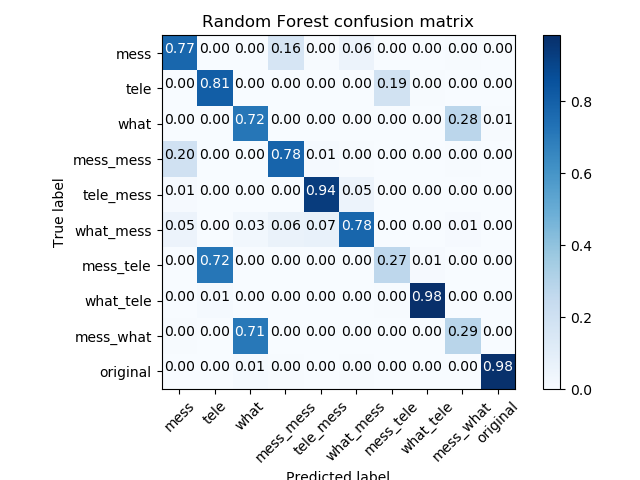
\includegraphics[scale=.6]{images/rf_initial_single_double_complete.png} 
\caption{random forest, last app classified} 
\end{figure} 


Result of the KFold validation with 10 bins:
 {\def\arraystretch{1.3} 
 \begin{table}[H] 
\centering 
\begin{tabular}{|l |l |l |l |l |l |l |l |l |l |}  
\hline 
0.7956&
0.8029&
0.7153&
0.8248&
0.6642&
0.8382&
0.7279&
0.7426&
0.6691&
0.7647\\ \hline  

\end{tabular} 
\end{table} }

The mean is : 0.754557
	\chapter{Double Scenario Classification of the last shared app, KFold Validation}Starting with fitting randomly the classifiers, there are some statistics of the data used for the first test: \\
 {\def\arraystretch{1.3} 
 \begin{table}[H] 
\centering 
\begin{tabular}{|l|l|l|} 
\hline 
  &count train  &count test  \\ \hline
messenger  &302  &748  \\ \hline
telegram  &314  &736  \\ \hline
whatsapp  &340  &710  \\ \hline
original  &94  &256  \\ \hline
\end{tabular} 
\end{table} }
\section{Logistic regression results:} 
Confusion matrix with number of sample and with normalization:
 {\def\arraystretch{1.3} 
 \begin{table}[H] 
\centering 
\begin{tabular}{|l|l|l|l|l|} 
\hline 
  &messenger  &telegram  &whatsapp  &original  \\ \hline
messenger  &746  &0  &2  &0  \\ \hline
telegram  &0  &618  &118  &0  \\ \hline
whatsapp  &0  &216  &494  &0  \\ \hline
original  &0  &0  &8  &248  \\ \hline
\end{tabular} 
\end{table} }

 \begin{figure}[H] 
\centering 
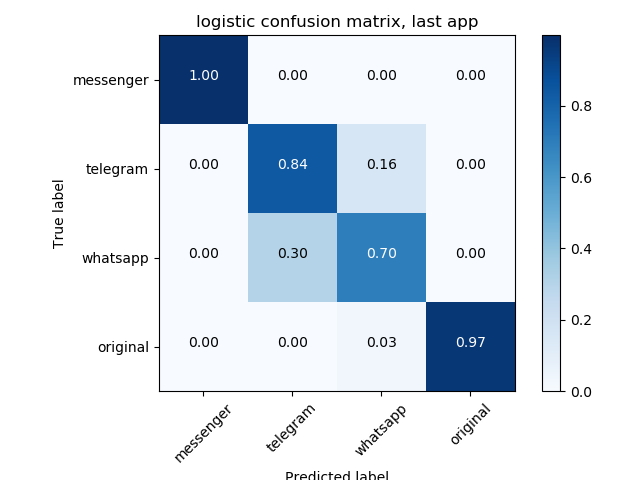
\includegraphics[scale=.6]{images/new_met_lr_initial_double_simple.png} 
\caption{logistic regression, last app classified} 
\end{figure} 


Result of the KFold validation with 10 bins:
 {\def\arraystretch{1.3} 
 \begin{table}[H] 
\centering 
\begin{tabular}{|l |l |l |l |l |l |l |l |l |l |}  
\hline 
0.8476&
0.8000&
0.9143&
0.8667&
0.8286&
0.8762&
0.8381&
0.8190&
0.8476&
0.8571\\ \hline  

\end{tabular} 
\end{table} }

The mean is : 0.849524\section{Linear Support Vector Machine results:} 
Confusion matrix with number of sample and with normalization:
 {\def\arraystretch{1.3} 
 \begin{table}[H] 
\centering 
\begin{tabular}{|l|l|l|l|l|} 
\hline 
  &messenger  &telegram  &whatsapp  &original  \\ \hline
messenger  &730  &6  &12  &0  \\ \hline
telegram  &0  &535  &201  &0  \\ \hline
whatsapp  &1  &197  &511  &1  \\ \hline
original  &0  &0  &6  &250  \\ \hline
\end{tabular} 
\end{table} }

 \begin{figure}[H] 
\centering 
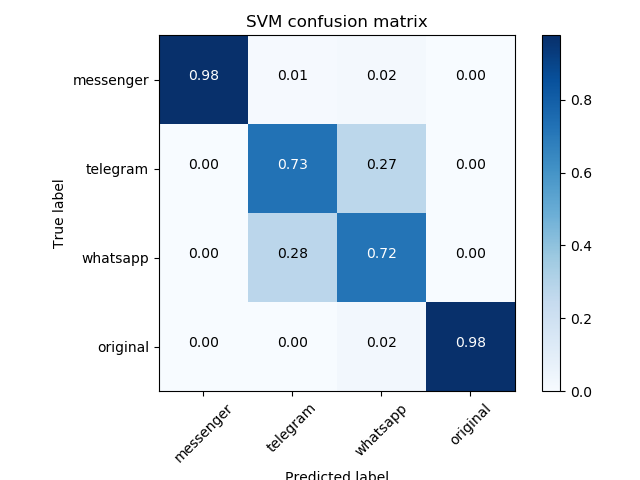
\includegraphics[scale=.6]{images/new_met_lsvm_initial_double_simple.png} 
\caption{linear SVM, last app classified} 
\end{figure} 


Result of the KFold validation with 10 bins:
 {\def\arraystretch{1.3} 
 \begin{table}[H] 
\centering 
\begin{tabular}{|l |l |l |l |l |l |l |l |l |l |}  
\hline 
0.8476&
0.8095&
0.8667&
0.7905&
0.7810&
0.8857&
0.8000&
0.8000&
0.8000&
0.8571\\ \hline  

\end{tabular} 
\end{table} }

The mean is : 0.823810\section{Random forest results:} 
Confusion matrix with number of sample and with normalization:
 {\def\arraystretch{1.3} 
 \begin{table}[H] 
\centering 
\begin{tabular}{|l|l|l|l|l|} 
\hline 
  &messenger  &telegram  &whatsapp  &original  \\ \hline
messenger  &740  &0  &8  &0  \\ \hline
telegram  &0  &627  &109  &0  \\ \hline
whatsapp  &1  &242  &463  &4  \\ \hline
original  &0  &0  &2  &254  \\ \hline
\end{tabular} 
\end{table} }

 \begin{figure}[H] 
\centering 
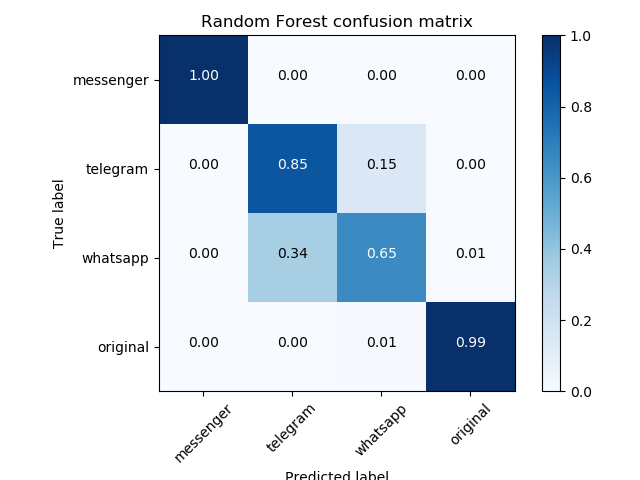
\includegraphics[scale=.6]{images/new_met_rf_initial_double_simple.png} 
\caption{random forest, last app classified} 
\end{figure} 


Result of the KFold validation with 10 bins:
 {\def\arraystretch{1.3} 
 \begin{table}[H] 
\centering 
\begin{tabular}{|l |l |l |l |l |l |l |l |l |l |}  
\hline 
0.8381&
0.8381&
0.8857&
0.9048&
0.8571&
0.8952&
0.8571&
0.8762&
0.8381&
0.8286\\ \hline  

\end{tabular} 
\end{table} }

The mean is : 0.861905
	

\chapter{Double Scenario Classification of the first and last shared app, KFold Validation}

Starting with fitting randomly the classifiers, there are some statistics of the data used for the first test: \\
 {\def\arraystretch{1.3} 
 \begin{table}[H] 
\centering 
\begin{tabular}{|l|l|l|} 
\hline 
  &count train  &count test  \\ \hline
mess\_mess  &96  &254  \\ \hline
tele\_mess  &99  &251  \\ \hline
what\_mess  &107  &243  \\ \hline
mess\_tele  &98  &252  \\ \hline
tele\_tele  &111  &239  \\ \hline
what\_tele  &105  &245  \\ \hline
mess\_what  &116  &234  \\ \hline
tele\_what  &103  &247  \\ \hline
what\_what  &121  &229  \\ \hline
original  &94  &256  \\ \hline
\end{tabular} 
\end{table} }
\section{Logistic regression results:} 
Confusion matrix with number of sample and with normalization:
 {\def\arraystretch{1.3} 
 \begin{table}[H] 
\centering 
\begin{tabular}{|l|l|l|l|l|l|l|l|l|l|l|} 
\hline 
  &m\_m  &m\_t  &m\_w  &t\_m  &t\_t  &t\_w  &w\_m  &w\_t  &w\_w  &original  \\ \hline
mess\_mess  &248  &5  &1  &0  &0  &0  &0  &0  &0  &0  \\ \hline
tele\_mess  &2  &233  &14  &0  &0  &0  &2  &0  &0  &0  \\ \hline
what\_mess  &13  &26  &202  &0  &0  &2  &0  &0  &0  &0  \\ \hline
mess\_tele  &0  &0  &0  &65  &116  &3  &0  &68  &0  &0  \\ \hline
tele\_tele  &0  &0  &0  &66  &57  &2  &0  &114  &0  &0  \\ \hline
what\_tele  &0  &0  &0  &3  &4  &235  &1  &2  &0  &0  \\ \hline
mess\_what  &0  &0  &0  &1  &0  &1  &80  &0  &152  &0  \\ \hline
tele\_what  &0  &0  &0  &65  &129  &3  &0  &50  &0  &0  \\ \hline
what\_what  &0  &0  &0  &0  &0  &0  &104  &0  &123  &2  \\ \hline
original  &0  &0  &0  &0  &0  &0  &0  &0  &5  &251  \\ \hline
\end{tabular} 
\end{table} }

 \begin{figure}[H] 
\centering 
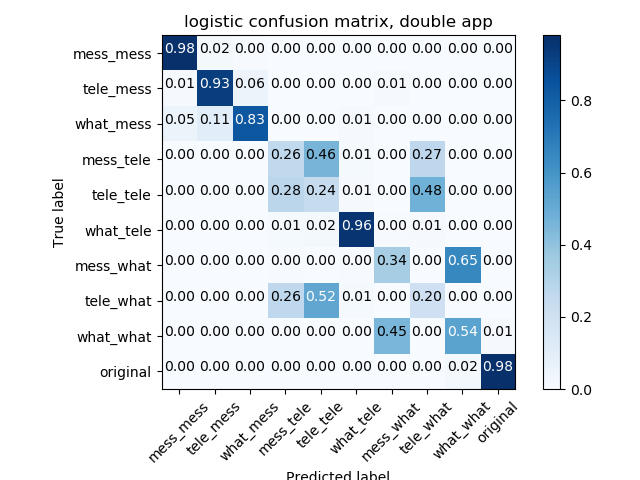
\includegraphics[scale=.6]{images/new_met_lr_initial_double_complete.png} 
\caption{logistic regression, last app classified} 
\end{figure} 


Result of the KFold validation with 10 bins:
 {\def\arraystretch{1.3} 
 \begin{table}[H] 
\centering 
\begin{tabular}{|l |l |l |l |l |l |l |l |l |l |}  
\hline 
0.6000&
0.5619&
0.6381&
0.6095&
0.6190&
0.6667&
0.6000&
0.5810&
0.5429&
0.6190\\ \hline  

\end{tabular} 
\end{table} }

The mean is : 0.603810\section{Linear Support Vector Machine results:} 
Confusion matrix with number of sample and with normalization:
 {\def\arraystretch{1.3} 
 \begin{table}[H] 
\centering 
\begin{tabular}{|l|l|l|l|l|l|l|l|l|l|l|} 
\hline 
  &m\_m  &m\_t  &m\_w  &t\_m  &t\_t  &t\_w  &w\_m  &w\_t  &w\_w  &original  \\ \hline
mess\_mess  &246  &4  &2  &0  &2  &0  &0  &0  &0  &0  \\ \hline
tele\_mess  &1  &213  &17  &2  &2  &0  &12  &1  &3  &0  \\ \hline
what\_mess  &14  &16  &194  &3  &0  &1  &7  &5  &3  &0  \\ \hline
mess\_tele  &0  &0  &0  &65  &105  &5  &0  &76  &1  &0  \\ \hline
tele\_tele  &0  &1  &0  &61  &52  &2  &0  &123  &0  &0  \\ \hline
what\_tele  &0  &0  &0  &3  &5  &232  &1  &4  &0  &0  \\ \hline
mess\_what  &0  &0  &0  &2  &2  &0  &78  &0  &152  &0  \\ \hline
tele\_what  &0  &1  &0  &58  &137  &3  &0  &48  &0  &0  \\ \hline
what\_what  &0  &0  &0  &1  &1  &0  &96  &1  &130  &0  \\ \hline
original  &0  &0  &0  &2  &1  &0  &0  &0  &5  &248  \\ \hline
\end{tabular} 
\end{table} }

 \begin{figure}[H] 
\centering 
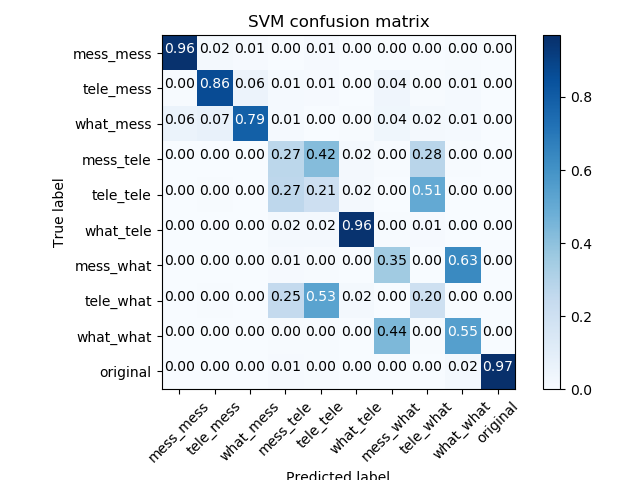
\includegraphics[scale=.6]{images/new_met_lsvm_initial_double_complete.png} 
\caption{linear SVM, last app classified} 
\end{figure} 


Result of the KFold validation with 10 bins:
 {\def\arraystretch{1.3} 
 \begin{table}[H] 
\centering 
\begin{tabular}{|l |l |l |l |l |l |l |l |l |l |}  
\hline 
0.6095&
0.5619&
0.6000&
0.5905&
0.6000&
0.6952&
0.6476&
0.5905&
0.5524&
0.6381\\ \hline  

\end{tabular} 
\end{table} }

The mean is : 0.608571\section{Random forest results:} 
Confusion matrix with number of sample and with normalization:
 {\def\arraystretch{1.3} 
 \begin{table}[H] 
\centering 
\begin{tabular}{|l|l|l|l|l|l|l|l|l|l|l|} 
\hline 
  &m\_m  &m\_t  &m\_w  &t\_m  &t\_t  &t\_w  &w\_m  &w\_t  &w\_w  &original  \\ \hline
mess\_mess  &235  &8  &8  &0  &0  &0  &2  &0  &0  &1  \\ \hline
tele\_mess  &16  &216  &19  &0  &0  &0  &0  &0  &0  &0  \\ \hline
what\_mess  &24  &26  &186  &0  &0  &0  &3  &0  &4  &0  \\ \hline
mess\_tele  &0  &0  &0  &36  &115  &4  &0  &97  &0  &0  \\ \hline
tele\_tele  &0  &0  &0  &80  &42  &5  &0  &112  &0  &0  \\ \hline
what\_tele  &0  &0  &0  &2  &1  &241  &0  &1  &0  &0  \\ \hline
mess\_what  &1  &0  &0  &0  &0  &0  &71  &0  &162  &0  \\ \hline
tele\_what  &0  &0  &0  &81  &125  &4  &0  &37  &0  &0  \\ \hline
what\_what  &0  &0  &0  &0  &0  &0  &133  &0  &92  &4  \\ \hline
original  &0  &0  &0  &0  &0  &1  &0  &0  &1  &254  \\ \hline
\end{tabular} 
\end{table} }

 \begin{figure}[H] 
\centering 
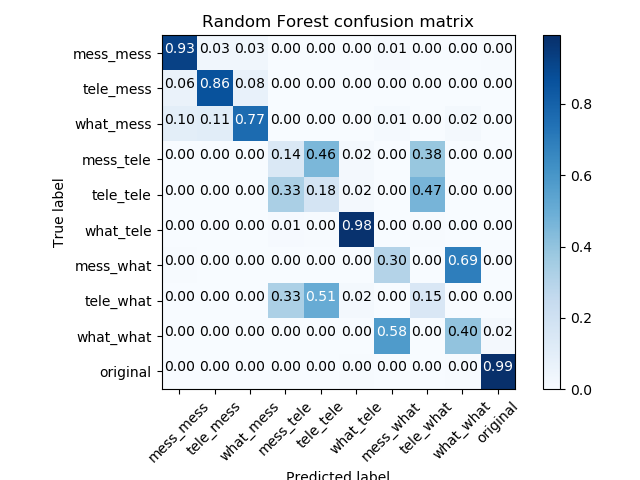
\includegraphics[scale=.6]{images/new_met_rf_initial_double_complete.png} 
\caption{random forest, last app classified} 
\end{figure} 


Result of the KFold validation with 10 bins:
 {\def\arraystretch{1.3} 
 \begin{table}[H] 
\centering 
\begin{tabular}{|l |l |l |l |l |l |l |l |l |l |}  
\hline 
0.5333&
0.5048&
0.6190&
0.5429&
0.5619&
0.6000&
0.5714&
0.6286&
0.4952&
0.5619\\ \hline  

\end{tabular} 
\end{table} }

The mean is : 0.561905
	

\chapter{Single and double scenario, KFold Validation}

Starting with fitting randomly the classifiers, there are some statistics of the data used for the first test: \\
 {\def\arraystretch{1.3} 
 \begin{table}[H] 
\centering 
\begin{tabular}{|l|l|l|} 
\hline 
  &count train  &count test  \\ \hline
mess  &97  &253  \\ \hline
tele  &335  &715  \\ \hline
what  &219  &481  \\ \hline
mess\_mess  &99  &251  \\ \hline
tele\_mess  &113  &237  \\ \hline
what\_mess  &93  &257  \\ \hline
mess\_tele  &89  &261  \\ \hline
what\_tele  &103  &247  \\ \hline
mess\_what  &106  &244  \\ \hline
original  &111  &239  \\ \hline
\end{tabular} 
\end{table} }
\section{Logistic regression results:} 
Confusion matrix with number of sample and with normalization:
 {\def\arraystretch{1.3} 
 \begin{table}[H] 
\centering 
\begin{tabular}{|l|l|l|l|l|l|l|l|l|l|l|} 
\hline 
  &m  &t  &w  &m\_m  &m\_t  &m\_w  &t\_m  &t\_w  &w\_m  &original  \\ \hline
mess  &184  &0  &0  &46  &4  &19  &0  &0  &0  &0  \\ \hline
tele  &0  &710  &0  &0  &0  &0  &0  &5  &0  &0  \\ \hline
what  &0  &0  &419  &0  &0  &0  &0  &0  &58  &4  \\ \hline
mess\_mess  &21  &0  &0  &220  &6  &4  &0  &0  &0  &0  \\ \hline
tele\_mess  &0  &0  &0  &0  &215  &22  &0  &0  &0  &0  \\ \hline
what\_mess  &0  &0  &0  &0  &88  &169  &0  &0  &0  &0  \\ \hline
mess\_tele  &0  &256  &0  &0  &0  &0  &0  &5  &0  &0  \\ \hline
what\_tele  &0  &9  &0  &0  &0  &0  &2  &236  &0  &0  \\ \hline
mess\_what  &0  &0  &191  &0  &0  &0  &0  &1  &52  &0  \\ \hline
original  &0  &0  &0  &0  &0  &0  &0  &0  &0  &239  \\ \hline
\end{tabular} 
\end{table} }

 \begin{figure}[H] 
\centering 
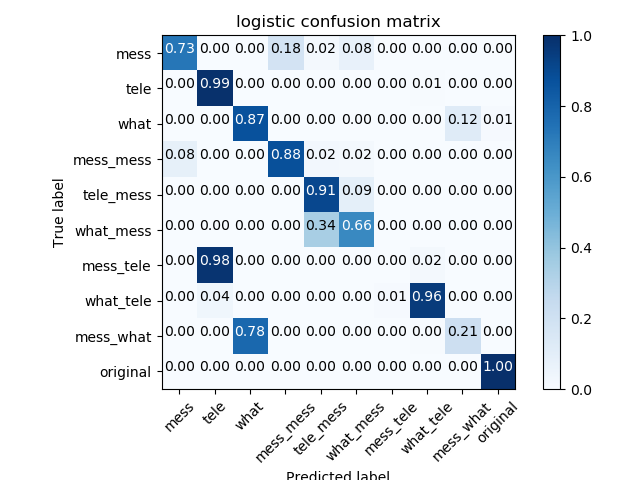
\includegraphics[scale=.6]{images/new_met_lr_initial_single_double_complete.png} 
\caption{logistic regression, last app classified} 
\end{figure} 


Result of the KFold validation with 10 bins:
 {\def\arraystretch{1.3} 
 \begin{table}[H] 
\centering 
\begin{tabular}{|l |l |l |l |l |l |l |l |l |l |}  
\hline 
0.8029&
0.7810&
0.7810&
0.7737&
0.7372&
0.7353&
0.7059&
0.8162&
0.7721&
0.7794\\ \hline  

\end{tabular} 
\end{table} }

The mean is : 0.768474\section{Linear Support Vector Machine results:} 
Confusion matrix with number of sample and with normalization:
 {\def\arraystretch{1.3} 
 \begin{table}[H] 
\centering 
\begin{tabular}{|l|l|l|l|l|l|l|l|l|l|l|} 
\hline 
  &m  &t  &w  &m\_m  &m\_t  &m\_w  &t\_m  &t\_w  &w\_m  &original  \\ \hline
mess  &192  &0  &0  &36  &5  &20  &0  &0  &0  &0  \\ \hline
tele  &0  &715  &0  &0  &0  &0  &0  &0  &0  &0  \\ \hline
what  &0  &0  &409  &0  &0  &0  &0  &0  &68  &4  \\ \hline
mess\_mess  &39  &0  &0  &204  &6  &2  &0  &0  &0  &0  \\ \hline
tele\_mess  &0  &0  &0  &0  &221  &16  &0  &0  &0  &0  \\ \hline
what\_mess  &0  &0  &0  &0  &66  &191  &0  &0  &0  &0  \\ \hline
mess\_tele  &0  &261  &0  &0  &0  &0  &0  &0  &0  &0  \\ \hline
what\_tele  &0  &5  &0  &0  &0  &0  &0  &242  &0  &0  \\ \hline
mess\_what  &0  &0  &174  &0  &0  &0  &0  &1  &69  &0  \\ \hline
original  &0  &0  &0  &0  &0  &0  &0  &0  &0  &239  \\ \hline
\end{tabular} 
\end{table} }

 \begin{figure}[H] 
\centering 
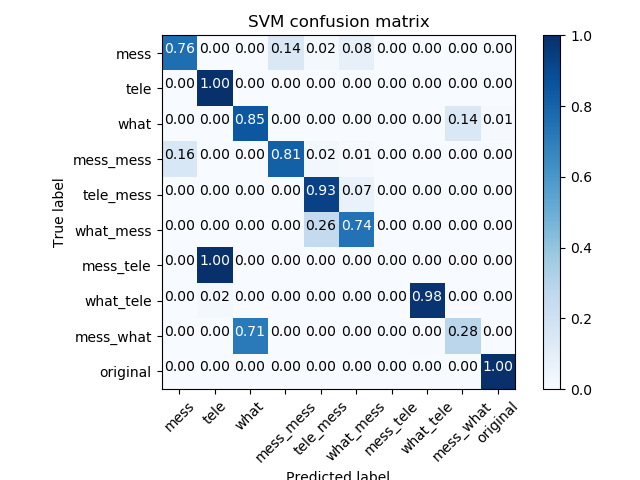
\includegraphics[scale=.6]{images/new_met_lsvm_initial_single_double_complete.png} 
\caption{linear SVM, last app classified} 
\end{figure} 


Result of the KFold validation with 10 bins:
 {\def\arraystretch{1.3} 
 \begin{table}[H] 
\centering 
\begin{tabular}{|l |l |l |l |l |l |l |l |l |l |}  
\hline 
0.8102&
0.7956&
0.7737&
0.8175&
0.7664&
0.8015&
0.7426&
0.8015&
0.8162&
0.7941\\ \hline  

\end{tabular} 
\end{table} }

The mean is : 0.791939\section{Random forest results:} 
Confusion matrix with number of sample and with normalization:
 {\def\arraystretch{1.3} 
 \begin{table}[H] 
\centering 
\begin{tabular}{|l|l|l|l|l|l|l|l|l|l|l|} 
\hline 
  &m  &t  &w  &m\_m  &m\_t  &m\_w  &t\_m  &t\_w  &w\_m  &original  \\ \hline
mess  &192  &0  &0  &36  &3  &19  &0  &0  &3  &0  \\ \hline
tele  &0  &609  &0  &0  &0  &0  &103  &3  &0  &0  \\ \hline
what  &0  &0  &362  &0  &0  &0  &0  &0  &115  &4  \\ \hline
mess\_mess  &50  &0  &0  &189  &8  &3  &0  &0  &1  &0  \\ \hline
tele\_mess  &1  &0  &0  &5  &211  &20  &0  &0  &0  &0  \\ \hline
what\_mess  &10  &0  &7  &17  &25  &196  &0  &0  &2  &0  \\ \hline
mess\_tele  &0  &199  &0  &0  &0  &0  &60  &2  &0  &0  \\ \hline
what\_tele  &0  &5  &0  &0  &0  &0  &1  &241  &0  &0  \\ \hline
mess\_what  &1  &0  &182  &0  &0  &0  &0  &0  &61  &0  \\ \hline
original  &0  &0  &5  &1  &0  &0  &0  &0  &0  &233  \\ \hline
\end{tabular} 
\end{table} }

 \begin{figure}[H] 
\centering 
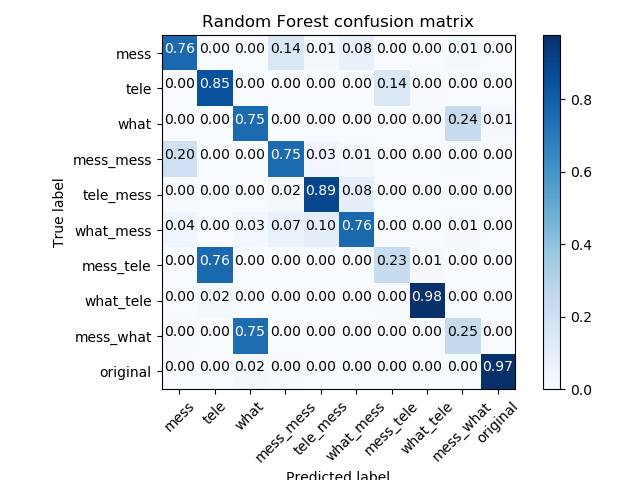
\includegraphics[scale=.6]{images/new_met_rf_initial_single_double_complete.png} 
\caption{random forest, last app classified} 
\end{figure} 


Result of the KFold validation with 10 bins:
 {\def\arraystretch{1.3} 
 \begin{table}[H] 
\centering 
\begin{tabular}{|l |l |l |l |l |l |l |l |l |l |}  
\hline 
0.7591&
0.7664&
0.7007&
0.7445&
0.6496&
0.8309&
0.7206&
0.7647&
0.6618&
0.7574\\ \hline  

\end{tabular} 
\end{table} }

The mean is : 0.735573
%	\input{new_methods.tex}
%	\input{conclusions.tex}
		
	\endgroup
	
	\addcontentsline{toc}{chapter}{Bibliografia}
	% stile con ordinamento alfabetico in funzione degli autori
	\bibliographystyle{plain}
	\bibliography{biblio}
	%\cellcolor{blue!25}
	
\end{document}